\section{Convergence of the out-forest}\label{sec.convoutforest}
In this section, we will show that the \L ukasiewicz path and height process corresponding to the forest $\hat{\cF}_n(m_n)$ converge under rescaling, for $m_n=O(n^{2/3})$. 
The main result of this section is as follows. 
\myworries{I think it is best to come up with new notation for $\sum_{i=1}^{m}\hat{D}^+_{n,i}$. Maybe $\hat{Y}^+_n(m)$? I will use that for now, and we can easily replace it later.}

\begin{theorem}\label{thm.convoutforest}
Like before, let $(\hat{\cF}_n(k),k\geq 1)$ be the sequence of out-forests given by the exploration, where we set $\hat{\cF}_n(k+1)=\hat{\cF}_n(k)$ if all half-edges have been paired at time $k$. Let $(\hat{S}^{+}_n(k),\hat{H}_n(k),k\geq 1)$ be the \L ukasiewicz path and height process corresponding to $(\hat{\cF}_n(k),k\geq 1)$. Let $\hat{S}^-_n(k)$ denote the number of unpaired in-half-edges of vertices that are seen at time $k$. Let $\hat{P}_n(k)$ be the number of purple vertices seen in the first $k$ time steps. \\
Moreover, let $(B_t)_{t\geq 0}$ be a Brownian motion, and define
$$(\hat{B}_t,t\geq 0):=\left( B_t-\frac{\sigma_{-+}+\nu_-}{2\sigma_+ \mu}t^2, t\geq 0\right).$$ 
Set $$(\hat{R}_t,t\geq 0)= \left(\hat{B}_t-\inf\left\{\hat{B}_s: s\leq t\right\},t\geq 0\right).$$
Then,

\begin{align*}\left(n^{-1/3}\hat{S}^{+}_n\left(\lfloor n^{2/3}t\rfloor \right),n^{-1/3}\hat{H}_{n}\left(\lfloor n^{2/3}t\rfloor \right), t\geq 0\right)
\overset{d}{\to}\left(\sigma_+ \hat{B}_t, \frac{2}{\sigma_+} \hat{R}_t, t\geq 0\right)\end{align*}
in $\D(\R_+,\R)^2$, and 
\begin{align*}\left( n^{-2/3}\hat{S}_n^-\left(\lfloor n^{2/3}t\rfloor \right), n^{-1/3}\hat{P}_n\left(\lfloor n^{2/3}t\rfloor \right), t\geq 0\right)\overset{p}{\to}\left(\nu_-t,  \frac{\nu_-}{2\mu} t^2, t\geq 0\right)\end{align*}
in $\D(\R_+,\R)^2$ as $n\to \infty$. 
\end{theorem}
\begin{remark}
Note that the sign of the parabolic drift is the same as the sign of $\mu-\E[D^+(D^-)^2]$, which is non-positive. Indeed,
$$\frac{\E[(Z^+)^2]}{\E[D^+]}-\left(\frac{\E[D^+D^-]}{\E[D^+]}\right)^2=\frac{\E[(Z^+)^2]}{\mu}-1$$
is the variance of $D^-$ under the law of $\mathbf{D}$ size-biased by $D^+$, which is non-negative. Hence $\E[D^+(D^-)^2]/\mu\geq 1$, which shows that $(\hat{B}_t)_{t\geq 0}$ is a Brownian motion with a downwards parabolic drift. 
\end{remark}
We prove Theorem \ref{thm.convoutforest} by studying two other forests that are related to $\hat{\cF}_n(m_n)$ via a change of measure.  \\
The proof is structured as follows.
\begin{enumerate}
    \item \label{item.measurechangeexists} Let $(\mathbf{\hat{D}}_{n,1},\dots,\mathbf{\hat{D}}_{n,n})$ denote the degree tuples in the order in which the corresponding vertices are included in the exploration. Fix $m$ and let $(\mathbf{Z}_1,\dots, \mathbf{Z}_m)$ be i.i.d. elements of $\N\times \N$, $\mathbf{Z}_i:=(Z_i^-,Z_i^+)$ such that 
    $$\P(Z_i^-=k^-, Z_i^+=k^+)=\frac{k^-\P(D^-=k^-,D^+=k^+)}{\mu}.$$
    Then, we show that the law of $(\mathbf{\hat{D}}_{n,1},\dots,\mathbf{\hat{D}}_{n,m})$ conditional on $\sum_{i=1}^n D_i^-=\sum_{i=1}^n D_i^+$ is absolutely continuous to $(\mathbf{Z}_1,\dots, \mathbf{Z}_m)$, and the Radon-Nikodym derivative $\phi_m^n$ is well-behaved for $m=O(n^{2/3})$. This is the content of Subsection \ref{subsec.measurechange}.
    \item Then, \ref{item.measurechangeexists} is the motivation to sample i.i.d. copies of $\mathbf{Z}$, $(\mathbf{Z}_i,i\geq 1)$, and to study a Galton-Watson forest with offspring distributed as $Z_1^+$. Call this forest $(\cF(k),k\geq 1)$. The convergence of the \L ukasiewicz path under scaling of $(\cF(k),k\geq 1)$ follows from Donsker's theorem.
    \item In Subsection XXX, we modify $(\cF(k),k\geq 1)$ to include purple leaves. We add extra randomness, such that at some time steps, a purple leaf is added. We call the resulting forest $(\cF^p_n(k),k\geq 1)$. We respect the order of the degrees in $(\cF(k),k\geq 1)$, in the sense that for any $k$, the $k^{th}$ black vertex in $(\cF^p_n(k),k\geq 1)$ has the same number of children as the $k^{th}$ vertex in $(\cF(k),k\geq 1)$. $(\cF^p_n(k),k\geq 1)$ depends on $n$, because the probability of finding a purple vertex depends on $n$. In Subsection XXX, we show that the \L ukasiewicz path and height process corresponding to $(\cF^p_n(k),k\geq 1)$ converge under rescaling, jointly with the convergence of the \L ukasiewicz path and height process corresponding to $(\cF(k),k\geq 1)$ under rescaling up to time $O(n^{2/3})$.
    \item We use the measure change to translate the convergence of the encoding processes of $(\cF^p_n(k),k\geq 1)$ under rescaling to convergence of the encoding processes of $(\hat{\cF}_n(k),k\geq 1)$ under rescaling up to time $O(n^{2/3})$. This yields Theorem \ref{thm.convoutforest}. 
\end{enumerate}

\subsection{The measure change and its convergence}\label{subsec.measurechange}
\myworries{Chapter 6 of Zheneng's transfer}

\subsection{Adding purple vertices to a Galton-Watson forest}
In this subsection we define $(\cF_n^p(k),k\geq 1)$  and show that its \L ukasiewicz path and height process converge under rescaling. Moreover, we will show that this convergence holds jointly with the convergence under rescaling of the number of purple vertices seen up to time $k$ and the number of seen, but unused in-half-edges up to time $k$.\\
Let $Y^+(k)=\sum_{i=1}^k (Z^+_i-1)$ be the \L ukasiewicz path corresponding to $(\cF(k),k\geq 1)$, and set $Y^-(k)=\sum_{i=1}^k (Z^-_i-1)$. Donsker's theorem and the strong law of large numbers imply that 
\begin{equation}\label{eq.convergenceGWforest}
    \left(n^{-1/3}Y^+\left(\lfloor n^{2/3}t \rfloor\right),n^{-2/3}Y^-\left(\lfloor n^{2/3}t \rfloor\right),t\geq 0\right)\overset{d}{\to} \left(\sigma_{-}B_t, \nu_-t, t\geq 0 \right)
\end{equation}
in $\D(\R_+,\R)^2$ as $n\to \infty$.\\
The following lemma motivates the definition of $(\cF_n^p(k),k\geq 1)$.
\begin{lemma}
Consider an eDFS of a configuration model on $n$ vertices, with the total number of in-half-edges equal to $\mu n$. Suppose the number of unpaired in-half-edges of discovered vertices at step $k$ in the exploration is equal to $S_n^{-}(k)$, suppose $(S_n^{+}(l),1\leq l\leq k)$ encodes the \L ukasiewicz path of the out-forest up to time $k$, and set $$I_n^{+}(k)=\inf\left\{S_n^{+}(l),1\leq l\leq k\right\}.$$
Then, the probability that, in the $(k+1)^{th}$ time step, we sample a surplus edge is given by
$$p_{k+1}:=\frac{S_n^{-}(k)}{\mu n - k -I^{+}(k)+1}\one_{\{I^{+}(k)=I^{+}(k-1)\}}.$$
\end{lemma}
\begin{proof}
This is a slight adaptation of Lemma \ref{lemma.sampleoutforest}, with $(\mathbf{\hat{D}}_{n,1},\dots,\mathbf{\hat{D}}_{n,m})$ replaced by $(\mathbf{Z}_1,\dots, \mathbf{Z}_m)$, and $\sum_{i=1}^n \hat{D}^-_i$ replaced by its mean $\mu n$.
\end{proof}

We will now define $(\cF_n^p(k),k\geq 1)$ and its \L ukasiewicz path $(S_n^{+}(k), k\geq 1)$ as a function of $(\cF(k),k\geq 1)$, $(Y^-(k),k\geq 1)$ and extra randomness.
\begin{enumerate} 
    \item Set $P_n(1)=0$, $S_n^{+}(1)=Z_1^+-1$, $S_n^{-}(1)=Z_1^-$. 
    \item Suppose we are given $(P_n(l),S_n^{+}(l),S_n^{-}(l), 1\leq l \leq k)$. Define 
    $I^{+}(k)=\min\{S_n^{+}(l), l\leq k\}$. Then, with probability $p_{k+1}$, independent from everything else, set $P_n(k+1)=P_n(k)+1$. Otherwise, set $P_n(k+1)=P_n(k)$. 
    \item Set $$S_n^{+}(k+1)=Y^+(k+1-P_n(k+1))-P_n(k+1),$$ and $$S_n^{-}(k+1)=Y^-(k+1-P_n(k+1))-P_n(k+1)-I^{+}(k)+1.$$
\end{enumerate}
Let $(\cF^p_n(k),k\geq 1)$ be the forest with \L ukasiewicz path $(S_n^{+}(k), k\geq 1)$ in which the $k^{th}$ vertex is purple if and only if $P^n(k)-P^n(k-1)=1$. 
\subsubsection{Convergence of the \L ukasiewicz path}
To show convergence of the \L ukasiewicz path corresponding to $(\cF^p_n(k),k\geq 1)$, we will first examine the limit of $(P_n(k), k\geq 1)$ under rescaling. We will first prove tightness, after which we will show convergence.


\begin{lemma}\label{lemma.tightnesssurplusedges}
 For every $T>0$, $$\left(n^{-1/3}P_n\left(\lfloor  n^{2/3}T\rfloor \right) \right)_{n\geq 1}$$ 
 is tight.
 \end{lemma}
 \begin{proof}
Set $m=\lfloor  n^{2/3}T\rfloor$ and fix $\epsilon>0$. It is trivial that for any $k\leq m$, $S^{-}(k)\leq \sum_{i=1}^k Z^-_i=Y^-(k)+k$. Moreover, $\mu n - k -I^{+}(l)+1>\mu n-k$.  Therefore, $$p_k\leq \frac{Y^-(k)+k}{\mu n - k},$$
and note that this upper bound is increasing in $k$. Consequently, conditional on $(Y^+(j),Y^-(j),j\geq 1),$ $n^{-1/3}P_n(m)$ is stochastically dominated by a binomial random variable with parameters  $m$ and $$\frac{Y^-(m)+m}{\mu n - m}\wedge 1.$$
Since $(Y^-(k)+k,k\geq 1)$ is a random walk with steps of finite mean, $\left(n^{-2/3}(Y^-(m)+m)\right)_{n\geq 1}$ is tight. Therefore,
$$\left(n^{1/3} \frac{Y^-(m)+m}{\mu n - m}\right)_{n\geq 1}$$ is tight, which proves the statement.
\end{proof}
\begin{lemma}\label{lemma.convergenceQandP}
We have that 
$$\left(n^{-1/3}P_n(\lfloor n^{2/3}t\rfloor), t \geq 0\right)\overset{p}{\to} \left(\frac{\nu_-}{2\mu} t^2, t\geq 0\right)$$
in $D(\R_+,\R)$ as $n\to \infty$.

\end{lemma}
\begin{proof}
Fix $T>0$. Recall that
$$p_{k+1}=\frac{S_n^{-}(k)}{\mu n - k -I^{+}(k)+1}\one_{\{I^{+}(k)=I^{+}(k-1)\}}.$$
Define $M(k)=\min\{Y^+(l):l\leq k\}$ such that $0\geq I^{+}(k)\geq M(k)-P_n(k)$.  Then, by Lemma \ref{lemma.tightnesssurplusedges}, Lemma  \eqref{eq.convergenceGWforest}, and the continuous mapping theorem, $\left(n^{-1/3}I^+(\lfloor n^{2/3} t \rfloor)\right)_{n\geq 1}$ is tight for all $t>0$.
We will now argue that the indicator, which ensures that the roots are never purple, does not have an effect on $(P_n(k),k\leq m)$ on the scale that we are interested in. Let $t>0$, and set $m=\lfloor n^{2/3}t\rfloor$. Define
\begin{align*}\begin{split}
E^p(m):&=\sum_{k=0}^{m-1}\frac{S_n^{-}(k)}{\mu n - k -I^{+}(k)+1}\one_{I^{+}(k)\neq I^{+}(k-1)}\\
&\leq I^{+}(m) \frac{Y^-(m)+m}{\mu n - m},\end{split}\end{align*}
so since $I^{+}(m)$ is of order $n^{1/3}$ and $\frac{Y^{-}(m)+m}{\mu n - m}$ is of order $n^{-1/3}$, $(E^p(m))_{n\geq 1}$ is tight for all $t\geq 0$.  This means that if we allow the roots to be purple, we would only sample $O(1)$ purple roots up to time $O(n^{2/3})$ with high probability, which does not affect $(P_n(k),k\leq m)$ on the scale that we are interested in. \\
 Then, the convergence in \eqref{eq.convergenceGWforest}, the tightness of $\left(n^{-1/3}I^{+}(\lfloor n^{2/3} t \rfloor)\right)_{n\geq 1}$ and Lemma \ref{lemma.tightnesssurplusedges} imply that
\begin{align}\begin{split}\label{eq.convergenceprob}
  &\left(n^{1/3}\frac{S_n^{-}\left(\lfloor n^{2/3} t \rfloor\right)}{\mu n - \lfloor n^{2/3} t \rfloor -I^{p,+}\left(\lfloor n^{2/3} t \rfloor\right)+1},t\geq 0\right)\\
 &=\left(n^{1/3}\frac{Y^-\left(\lfloor n^{2/3} t \rfloor-P_n\left(\lfloor n^{2/3} t \rfloor\right)\right)-P_n\left(\lfloor n^{2/3} t \rfloor\right)-I^{+}\left(\lfloor n^{2/3} t \rfloor\right)+1}{\mu n - \lfloor n^{2/3} t \rfloor -I^{+}\left(\lfloor n^{2/3} t \rfloor\right)+1},t\geq 0\right)\\
 &\overset{p}{\to} \left(\frac{\nu_-}{\mu}t,t\geq 0\right)\end{split}\end{align}
in $D(\R_+,\R)$ as $n\to \infty$. 
Then, by the continuous mapping theorem and the tightness of $(E^p(m))_{n\geq 1}$,
$$\left(n^{-1/3}\sum_{i=0}^{\lfloor n^{2/3}t \rfloor} p_k , t \geq 0\right)\overset{p}{\to} \left(\frac{\nu_-}{2\mu}t^2,t\geq 0\right)$$
in $D(\R_+,\R)$ as $n\to \infty$. \\
Let $\cG=(\cG_k,k\geq 1)$ denote the filtration such that $\cG_{k}$ contains the information on the shape of the forest until time $k$, including the colours of the vertices. Then, 
$$M_n(k):=\sum_{i=1}^k (\one_{\{P_n(i)-P_n(i-1)=1\}}-p_i)$$ is a martingale in $\cG$. We claim that $(n^{-1/3}M_n(\lfloor n^{2/3} t\rfloor ), t\geq 0)$ converges to $(0,t\geq 0)$ in probability in $D(\R_+,\R)$. Indeed, for any $t\geq 0$,
\begin{align*}\E[n^{-2/3}M_n(\lfloor n^{2/3} t\rfloor )^2]&=n^{-2/3}\sum_{i=1}^{\lfloor n^{2/3} t\rfloor} \E[\E[(\one_{\{P_n(i)-P_n(i-1)=1\}}-p_i)^2|\cG_{i-1}]]\\&=n^{-2/3}\sum_{i=1}^{\lfloor n^{2/3} t\rfloor} \E[p_i-p_i^2]\to 0.\end{align*}
Hence,
$$\left(n^{-1/3}P_n(\lfloor n^{2/3}t\rfloor), t\geq 0\right)=\left(n^{-1/3}\sum_{i=1}^{\lfloor n^{2/3}t\rfloor}  \one_{\{P_n(i)-P_n(i-1)=1\}}  , t\geq 0\right)\overset{d}{\to} \left( \frac{\nu_-}{2\mu}t^2, t\geq 0 \right),$$
 which proves the statement.

\end{proof}

The convergence of $P_n$ under rescaling implies the convergence of $S^{+}$ and $S^{-}$ under rescaling, which is the content of the following corollary. 

\begin{corollary}\label{cor.lukasiewiczpathpurplevertices}
 Let $(B_t,t\geq 0)$ be a Brownian motion. We have that 
 \begin{align*}\left(n^{-1/3}Y^{+}\left(\lfloor n^{2/3}t\rfloor\right), n^{-1/3}S^{+}_n\left(\lfloor n^{2/3}t\rfloor\right), t\geq 0\right)\overset{d}{\to}\left(\sigma_+B_t,\sigma_+B_t-\frac{\nu_-}{2\mu}t^2,  t\geq 0\right)\end{align*}
 in $\D(\R_+,\R)^2$  and 
 $$\left(n^{-2/3}S^{-}_n\left(\lfloor n^{2/3}t\rfloor\right),t\geq 0\right)\overset{p}{\to}\left(\nu_- t,t\geq 0\right)$$
 in $\D(\R_+,\R)$ as $n\to\infty$.
\end{corollary}
\begin{proof}
 This follows from \eqref{eq.convergenceGWforest}, Lemma \ref{lemma.convergenceQandP} and the expressions 
 $$S_n^{p,+}(k+1)=Y^+(k+1-P_n(k+1))-P_n(k+1),$$ and $$S_n^{p,-}(k+1)=Y^-(k+1-P_n(k+1))-P_n(k+1)-I^{p,+}(k)+1.$$
\end{proof}

\subsubsection{Convergence of the height process}\label{subsubsec.convheightprocess}
We will extend Corollary \ref{cor.lukasiewiczpathpurplevertices} to joint convergence under rescaling with the height process corresponding to $(\cF^p_n(k),k\geq 1)$, which is the content of this subsubsection. We prove the following proposition. 
\begin{proposition}\label{prop.convheightprocesspurple}
Let $(H^{+}(k),k\geq 1)$ be the height process corresponding to $(\cF^p(k),k\geq 1)$. Let $(B_t,t\geq 0)$ be a Brownian motion, and define 
$$({B}^+_t,t\geq 0)=\left(B_t-\frac{\nu_-}{2\mu\sigma_+}t^2,t\geq 0\right).$$ 
Set $$(R^+_t,t\geq 0)=\left({B}^+_t-\inf\left\{{B}^+_s: s\leq t\right\},t\geq 0 \right).$$
Then,

\begin{align*}&\left(n^{-1/3}Y^{+}\left(\lfloor n^{2/3}t\rfloor\right), n^{-1/3}S^{+}_n\left(\lfloor n^{2/3}t\rfloor\right),n^{-1/3}H^{+}_n\left(\lfloor n^{2/3}t\rfloor\right), t\geq 0\right) \overset{d}{\to}\left(\sigma_+B_t,\sigma_+{B}^+_t, \frac{2}{\sigma_+} R^+_t,  t\geq 0\right)\end{align*}
 in $\D(\R_+,\R)^3$, and 
 $$\left(n^{-2/3}S^{-}_n\left(\lfloor n^{2/3}t\rfloor\right),t\geq 0\right)\overset{p}{\to}\left(\nu_- t,t\geq 0\right)$$
 in $\D(\R_+,\R)$ as $n\to\infty$.
\end{proposition}
The difficulty in proving this proposition is the fact that $(\cF^p_n(k),k\geq 1)$ is not a Galton-Watson forest, because the probability of sampling a purple leaf changes as time progresses. In fact, the sampling process does not even satisfy the Markov property, because the probability of sampling a purple vertex depends on the past of the process. The theory of convergence of height processes under rescaling for Galton-Watson forests is a well-developed (see e.g. \cite{Duquesne2005}), but this is not the case for more general processes.  We will adapt a technique that Broutin, Duquesne and Wang develoved in \cite{Broutin2020} to show convergence of the height process of inhomogeneous random graphs under rescaling. The key idea is that  $(\cF^p_n(k),k\geq 1)$ itself is not a Galton-Watson forest, but we can embed it in a Galton-Watson forest, say $(\cF^{pr}(k),k\geq 1)$, which will be equal to $(\cF^p_n(k),k\geq 1)$ with extra red vertices. We then show convergence under rescaling of the height process corresponding to $(\cF^{pr}(k),k\geq 1)$, and use this to obtain height process convergence for $(\cF^p_n(k),k\geq 1)$. \\
We start by defining $(\cF^{pr}(k),k\geq 1)$. Informally, we obtain $(\cF^{pr}(k),k\geq 1)$ by modifying $(\cF^p_n(k),k\geq 1)$ in such a way that the sub-tree rooted at a purple vertex has the same law as a sub-tree rooted at a black vertex. We do this by sampling extra Galton Watson trees with offspring distributed as $Z^+$, of which we colour all vertices red, and identifying their roots with the purple vertices. The resulting forest is a black-purple-red Galton-Watson forest in which the black-purple forest is embedded. This is illustrated in Figure \ref{fig.blackpurpleredforest}. 

\begin{figure}
    \centering
    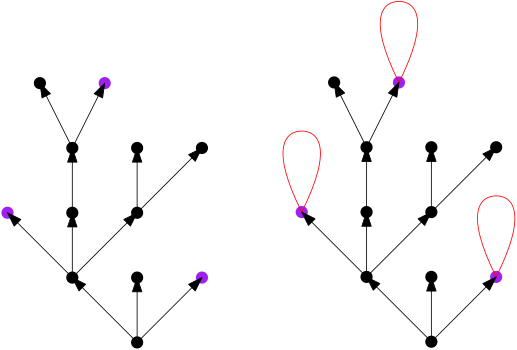
\includegraphics[scale=0.6]{Content/Pictures/black-purple-red tree.png}
    \caption{Given a component of $(\cF^p_n(k),k\geq 1)$ (see left figure), we modify it by sampling independent red Galton-Watson trees with offspring distributed as $Z^+$ and identifying each purple vertex with a root of a red tree. The resulting tree (see right figure) is a Galton-Watson tree, and the resulting forest $(\cF^{pr}_n(k),k\geq 1)$ is a Galton-Watson forest.}
    \label{fig.blackpurpleredforest}
\end{figure}
The formal procedure is as follows. Suppose we are given $(Y^+(k),S^{+}(k),P_n(k),k\geq 1)$, which encode $(\cF^p_n(k),k\geq 1)$.
\begin{enumerate}
    \item Let $(Y^{red}(k),k\geq 1)$ be an independent copy of $(Y^+(k),k\geq 1)$. $(Y^{red}(k),k\geq 1)$ will encode the red pendant subtrees. 
    \item Define $\theta_n(k)=k+\min\{j: Y^{red}(j)=-P_n(k-1)\}-P_n(k-1)$. 
    \item Set $\Lambda_n(k)=\max\{j:\theta_n(j)\leq k\}-P_n(\max\{j:\theta_n(j)\leq k\})$. 
    \item We now define \begin{equation}\label{eq.definitionY^{pr}}(Y^{pr}(k),k\geq 1)=(Y^+(\Lambda_n(k))+Y^{red}(k-\Lambda_n(k)),k\geq 1)\end{equation}
    and we let $(\cF^{pr}(k),k\geq 1)$ be the Galton-Watson process encoded by $(Y^{pr}(k),k\geq 1)$, in which $P_n(\max\{j:\theta_n(j)\leq k\})$ of the first $k$ vertices are blue, $\Lambda_n(k)$ of the first $k$ vertices are black, and the rest is red. We let $(H^{pr}(k),k\geq 1)$ be the height process corresponding to $(\cF^{pr}(k),k\geq 1)$.
\end{enumerate}
We claim that the forest consisting of the black and blue vertices in $\cF^{pr}(\theta_n(k))$ is, by construction, equal to $\cF^{p}(k)$. Moreover, $(\cF^{pr}(k),k\geq 1)$ is a Galton-Watson forest. We make the following observations.
\begin{enumerate}
    \item We claim that $$\theta_n(k)=\min\{l: \cF^p(k)\text{ is a subforest of }\cF^{pr}(l)\}.$$ Indeed, note that $\min\{j: Y^{red}(j)=-P_n(k-1)\}$ is equal to the number of vertices in the first $P_n(k-1)$ trees in the forest encoded by $Y^{red}$, so $$\min\{j: Y^{red}(j)=-P_n(k-1)\}-P_n(k-1)$$ is equal to the number of red vertices we add to $\cF^p(k)$. Then, $\theta_n(k)$ is the index in $(\cF^{pr}(k),k\geq 1)$ of the $k^{th}$ black or purple vertex. 
    \item Note that $\Lambda_n(k)$ is the number of blue vertices amongst the first $k$ vertices. This follows from the fact that $\max\{j:\theta_n(j)\leq k\}$ is the number of blue or purple vertices amongst the first $k$ vertices. 
    \item By the argument above, $(\Lambda_n(k),k\geq 1)$ only takes steps of size $0$ or $1$. Both $(Y^+(k),k\geq 1)$ and $(Y^{red}(k),k\geq 1)$ are random walks with steps distributed as $Z^+-1$, so, by construction, $(Y^{pr}(k),k\geq 1)$ is a random walk with steps distributed as $Z^+-1$, so $(\cF^{pr}(k),k\geq 1)$ is a Galton-Watson forest with offspring distributed as $Z^+$.
    \item By construction, $(H^{pr}(\theta_n(k)),k\geq 1)$ is the height process corresponding to $(\cF^p_n(k),k\geq 1)$. Moreover,
   \begin{equation}\label{eq.constructionSp}(S^{+}(k),k\geq 1)=(Y^{pr}(\theta_n(k))-E(\theta_n(k)),k\geq 1),\end{equation}
    where 
    $E(k)$ counts the red children of the $k^{th}$ vertex in $(\cF^{pr}(k),k\geq 1)$.
\end{enumerate}
Considering the construction above and Corollary \ref{cor.lukasiewiczpathpurplevertices}, in order to prove Proposition \ref{prop.convheightprocesspurple}, it is sufficient to show that there exists a process $(D_t,t\geq 0)$ such that 
\begin{align}\begin{split}\label{eq.convergenceSpr}
    &\left(n^{-1/3}\left(Y^{pr}\left(\theta_n\left(\lfloor n^{2/3}t\rfloor \right)\right)-E\left(\lfloor n^{2/3}t\rfloor \right)\right), n^{-1/3}H^{pr}\left(\theta_n\left(\lfloor n^{2/3}t\rfloor \right)\right),t\geq 0\right)\\
    &\overset{d}{\to}\left(\sigma_+D_t,\frac{2}{\sigma_+}\left(D_t-\inf\left\{D_s,s\leq t\right\}\right),t\geq 0\right)
\end{split}\end{align}
in $\D(\R_+,\R)^2$ as $n\to \infty$ and $\left(\frac{2}{\sigma_+}\left(D_t-\inf\left\{D_s,s\leq t\right\}\right),t\geq 0\right)$ is the height process corresponding to $(\sigma_+D_t,t\geq 0)$. 

The next lemma show that the pathwise construction of $(Y^{pr}(k),H^{pr}(k),k\geq 1)$ converges to the continuous counterpart of the pathwise construction.

\begin{lemma}\label{lemma.convergenceX+}
Let $(B_t, t \geq 0)$ and $(B^{red}_t, t\geq 0)$ be two independent Brownian motions and let $$\theta(t):=t+\inf\left\{s\geq 0 : \sigma_+ B^{red}_s< -\frac{\nu_-}{2\mu} t^2\right\},$$ and $\Lambda(t)=\inf\{s\geq 0:\theta(s)> t\}$. Define \begin{equation}\label{eq.definitionBpr}\left(B^{pr}_t,t \geq 0\right):=\left( B_{\Lambda(t)}+ B^{red}_{t-\Lambda(t)}, t\geq 0\right).\end{equation}
Then, for $$(R^{pr}_t, t\geq 0):=\left(B^{pr}_t-\inf\{B^{pr}_s,s\leq t\},t\geq 0\right),$$
$\left((2/\sigma_+)R^{pr}_t, t\geq 0\right)$
is the height process corresponding to $\left(\sigma_+ B^{pr}_t,t \geq 0\right)$.
Moreover,

\begin{equation}\label{eq.convergenceYpr} \left(n^{-1/3}Y^{pr}\left( \lfloor n^{2/3}t \rfloor \right), n^{-1/3}H^{pr}\left( \lfloor n^{2/3}t \rfloor \right),t\geq 0\right)\overset{d}{\to}\left( \sigma_+ B^{pr}_{t} ,\frac{2}{\sigma_+}R^{pr}_t, t\geq 0\right)\end{equation}
in $D(\R_+,\R)^2$, jointly with 
$$\left(n^{-1/3}Y^+\left(\lfloor n^{2/3}t \rfloor \right), n^{-1/3}Y^{red}\left(\lfloor n^{2/3}t \rfloor \right), t\geq 0\right) \overset{d}{\to}\left(\sigma_+ B_t,\sigma_+ B^{red}_t, t\geq 0\right)$$
in $D(\R_+,\R)^2$ and 
$$\left(n^{-2/3} \Lambda_n\left(\lfloor n^{2/3}t\rfloor \right), n^{-2/3}\theta_n\left(\lfloor n^{2/3}t\rfloor \right),t\geq 0\right)\overset{d}{\to}\left(\Lambda(t),\theta(t), t\geq 0 \right)$$
in $D(\R_+,\R)^2$ as $n\to \infty$. 
In particular, 
\begin{equation}\label{eq.convergencecompSprandtheta}\left(n^{-1/3}Y^{pr}\left(\theta_n \left(\lfloor n^{2/3}t\rfloor \right)\right), n^{-1/3}H^{pr}\left(\theta_n\left(\lfloor n^{2/3}t\rfloor \right) \right),t\geq 0 \right) \overset{d}{\to} \left(\sigma_+ B^{pr}_{\theta(t)}, \frac{2}{\sigma_+}R^{pr}_{\theta(t)},t\geq 0\right)\end{equation}
in $D(\R_+,\R)^2$ as $n\to \infty$ jointly with the convergence above.
\end{lemma}
In the proof of Lemma \ref{lemma.convergenceX+} we use the following, straightforward, technical result. 

\begin{lemma}\label{lemma.technicalcomposedfunctions}
If $h_n\to h$ and $f_n\to f$ in $\D(\R_+,\R)$ as $n\to\infty$, and $h_n$ and $h$ are monotone non-decreasing and $h$ is continuous, then 
$$h_n\circ f_n \to h\circ f$$
and 
$$f_n\circ h_n \to f\circ h$$
in $\D(\R_+,\R)$ as $n\to\infty$.
\end{lemma}
\begin{proof}
Using the characterization of convergence in the Skorokhod topology given in Proposition 3.6.5 in \cite{Ethier1986} by Ethier and Kurtz, the result follows immediately.
\end{proof}


\begin{proof}[of \emph{Lemma \ref{lemma.convergenceX+}}]
Firstly, note that by $(Y^{pr}(k),k\geq 1)$ encoding a critical Galton-Watson forest with offspring variance $\sigma_+^2$, the proof of Theorem 1.8 in \cite{Legall2005} gives us that for $(B^*_s,s\geq 0)$ a Brownian motion,
\begin{equation}\label{eq.convergenceX}\left(n^{-1/3}Y^{pr}\left(\lfloor n^{2/3}s\rfloor \right), n^{-1/3}H^{pr}\left(\lfloor n^{2/3}s\rfloor \right), s\geq 0 \right) \overset{d}{\to} \left(\sigma_+ B^*_s,\frac{2}{\sigma_+} \left(B^*_s-\inf\{B^*_u:u\leq s\}\right),  s\geq 0\right) \end{equation}
 in $D(\R_+,\R)^2$ as $n\to \infty$, and $\left(\frac{2}{\sigma_+}(B^*_s-\inf\{B^*_u,u\leq s\}),s\geq 0\right)$ is the height process corresponding to $\left(\sigma_+ B^*_s,s \geq 0\right)$. Moreover, \cite{Chaumont2010} and the fact that $(Y^+(k),k\geq 1)\overset{d}{=}(Y^{red}(k),k\geq 1)\overset{d}{=}(Y^{pr}(k),k\geq 1)$ imply that
\begin{align}\begin{split}\label{eq.convergencebychaumont}&\left(n^{-1/3}Y^{red}\left(\lfloor n^{2/3} s \rfloor \right), n^{-2/3}\inf\left\{k:n^{-1/3}Y^{red}(k) \leq -x\right\}, s \geq 0, x\geq 0 \right)\\
&\overset{d}{\to}\left( \sigma_+ B^{red}_s, \inf\left\{u:\sigma_+ B^{red}_u < -x\right\}, s\geq 0, x \geq 0\right)\end{split}\end{align}
in $D(\R_+,\R)^2$ and 
$$\left(n^{-1/3}Y^+\left(\lfloor n^{2/3} t\rfloor \right),t\geq 0\right)\overset{d}{\to}\left(\sigma_+ B_t, t\geq 0\right)$$
in $D(\R_+,\R)$ as $n\to \infty$. Moreover, it is standard that 
\begin{equation}\label{eq.hittingtimestableprocess}\left(\inf\left\{u:\sigma_+ B^{red}_u < -x\right\},x\geq 0\right)\overset{d}{=}\left(\frac{1}{\sigma_+^2}L_x,x\geq 0\right),\end{equation}
with $(L_x,x\geq 0)$ a stable subordinator with exponent $1/2$.
Since $(P_n(k),k\geq 1)$ is non-decreasing, applying Lemma \ref{lemma.technicalcomposedfunctions}, and combining the convergence in \eqref{eq.convergencebychaumont} with Lemma \ref{lemma.convergenceQandP} gives that also
$$\left(n^{-2/3}\inf\left\{k:Y^{red}(k) \leq - P_n\left(\lfloor n^{2/3} t \rfloor -1\right)\right\},t\geq 0\right)\overset{d}{\to}\left(\inf\left\{u:\sigma_+ B^{red}_u< -\frac{\beta - \mu}{2\mu^2} t^2\right\},t\geq 0\right)$$
  in $D(\R_+,\R)$ as $n\to \infty$ jointly with the convergence in \eqref{eq.convergencebychaumont},
  and therefore, 
 \begin{equation}\label{eq.convergencetheta}\left(n^{-2/3}\theta_n\left(\lfloor n^{2/3}t\rfloor \right),t\geq 0 \right) \overset{d}{\to} \left(\theta(t),t\geq 0\right)\end{equation}
  in $D(\R_+,\R)$ as $n\to \infty$ jointly with the convergence in \eqref{eq.convergencebychaumont}.
Recall that 
$$\Lambda_n(k)=\max\{j:\theta_n(j)\leq k\}-P_n(\max\{j:\theta_n(j)\leq k\}). $$ By \eqref{eq.hittingtimestableprocess}, the jumps of $\left(\theta(t),t\leq T\right)$ are dense, and since $(\theta_n(k),k\geq 1)$ is increasing for all $n$ and $(\theta(t),t\geq 0)$ is increasing,  
$$\left(n^{-2/3}\max\{j:\theta_n(j)\leq \lfloor n^{2/3} t \rfloor\} ),t\geq 0\right)\overset{d}{\to}\left( \Lambda(t),t\geq0 \right)$$
in $D(\R_+,\R)$ as $n\to \infty$ jointly with the convergence in \eqref{eq.convergencebychaumont} and \eqref{eq.convergencetheta}. Since $\max\{j:\theta_n(j)\leq \lfloor n^{2/3} t \rfloor\}$ is of order $n^{2/3}$, Lemma \ref{lemma.tightnesssurplusedges} implies that also 
$$\left(n^{-2/3}\Lambda_n\left(\lfloor n^{2/3} t \rfloor\} \right),t\geq 0\right)\overset{d}{\to}\left( \Lambda(t),t\geq0 \right)$$
in $D(\R_+,\R)$ as $n\to \infty$ jointly with the convergence in \eqref{eq.convergencebychaumont} and \eqref{eq.convergencetheta}.\\
To finish the proof, we examine the construction of $(Y^{pr}(k),k\geq 1)$ in \eqref{eq.definitionY^{pr}} and the construction of $(B^{pr}_s,s\geq 0)$ in \eqref{eq.definitionBpr}. 
Note that $\Lambda_n(k)$ and $k-\Lambda_n(k)$ are non-decreasing. Again, by Lemma \ref{lemma.technicalcomposedfunctions}, this implies that 
$$\left(n^{-1/3}Y^{pr}\left( \lfloor n^{2/3} t \rfloor \right), t\geq 0 \right)\overset{d}{\to} \left( B^{pr}_{t}, t\geq 0\right)$$
in $D(\R_+,\R)$ as $n\to \infty$ jointly with all earlier mentioned converging random variables. Combining this with the convergence in \eqref{eq.convergenceX} proves \eqref{eq.convergenceYpr}. The fact that $(\theta_n(k),k\geq 1)$ is non-decreasing and Lemma \ref{lemma.technicalcomposedfunctions} then imply \eqref{eq.convergencecompSprandtheta}. 
\end{proof}

\begin{lemma}\label{lemma.subtracterrorconverges}
We have that 
$$\left(n^{-1/3}S^{+}\left(\lfloor n^{2/3}t\rfloor \right)), n^{-1/3}H^{+}\left(\lfloor n^{2/3}t\rfloor \right) ,t\geq 0 \right) \overset{d}{\to} \left(\sigma_+ B^{pr}_{\theta (t)},\frac{2}{\sigma_+} \left(B^{pr}_{\theta (t)}-\inf\{B^{pr}_{s}:s\leq \theta(t)\}\right) ,t\geq 0 \right)$$
in $D(\R_+,\R)^2$ as $n\to \infty$. 
\end{lemma}


\begin{proof}
By \eqref{eq.constructionSp}, and by Lemma \ref{lemma.convergenceX+}, it is sufficient to show that for any $T>0$,
$$n^{-1/3}\max_{k\leq \lfloor n^{2/3}T\rfloor}E(k)\overset{p}{\to}0.$$
We remind the reader that $E(k)$ counts the number of red children of $k^{th}$ vertex in $(\cF^{pr}(k),k\geq 1)$, so
$$n^{-1/3}\max_{k\leq \lfloor n^{2/3}T\rfloor}E(k)\leq n^{-1/3}\max_{k\leq \theta_n(\lfloor n^{2/3}T\rfloor)}(Y^{red}(k)-Y^{red}(k-1)+1),$$
which converges to $0$ by tightness of $\left(n^{-2/3}\theta^{n}(\lfloor n^{2/3}T\rfloor)\right)_{n\geq 1}$ and the fact that $$\left(n^{-1/3}Y^{red}\left(\lfloor n^{2/3}t\rfloor\right),t\geq 0\right)$$ converges in distribution to a continuous process in $D(\R_+,\R)$ as $n\to\infty$.
\end{proof}

The following lemma is the last ingredient in the proof of \eqref{eq.convergenceSpr}, and therefore also in the proof of Proposition  \ref{prop.convheightprocesspurple}. 
\begin{lemma}\label{lemma.heightprocesstimechange}
We have that with probability $1$, $$\left(\frac{2}{\sigma_+} \left(B^{pr}_{\theta (t)}-\inf\{B^{pr}_{s}:s\leq \theta(t)\}\right), t\leq T \right)=\left(\frac{2}{\sigma_+} \left(B^{pr}_{\theta (t)}-\inf\{B^{pr}_{\theta(s)}:s\leq t\}\right), t\leq T \right),$$ which is continuous, and it is the height process corresponding to $\left(\sigma_+ B^{pr}_{\theta (t)},t\leq T\right)$. 
\end{lemma}
\begin{proof}
From \cite{Legall2005}, we know that $\left(\frac{2}{\sigma_+}R^{pr}_t,t\geq 0\right)$ is the height process corresponding to $\left(\sigma_+ B^{pr}_{t},t\geq 0\right)$. By definition of the height process, we prove the statement if we show that with probability $1$, $(B^{pr}_{\theta(t)},t\geq 0)$ is continuous, and for all $t\geq 0$, for all $s$ such that $\theta(t-)<s<\theta(t)$, $ B^{pr}_s > B^{pr}_{\theta(t)}$. \\
Recall that $(B_t, t \geq 0)$ and $(B^{red}_t, t\geq 0)$ are two independent Brownian motions, $$\theta(t)=t+\inf\left\{s\geq 0 : \sigma_+ B^{red}_s< -\frac{\nu_-}{2\mu} t^2\right\},$$ and $\Lambda(t)=\inf\{s\geq 0:\theta(s)> t\}$. Then, \begin{equation*}\left(B^{pr}_t,t \geq 0\right):=\left( B_{\Lambda(t)}+ B^{red}_{t-\Lambda(t)}, t\geq 0\right).\end{equation*}
Firstly, note that the jumps of $\theta$ correspond to excursions above the infimum of $B^{red}$.  With probability $1$, for all these excursions, the minimum on the excursion is only attained at the endpoints. This can be seen by uniqueness of local minima of Brownian motion. We will assume that this holds.\\
Now fix $t$ such that $\theta(t-)\neq \theta(t)$ and let $s\in (\theta(t-),\theta(t))$. Observe that $\Lambda$ is equal to $t$ on $[\theta(t-),\theta(t)]$. For $[\theta(t-),\theta(t))$ this follows by definition of $\Lambda$, and for $\theta(t)$ this follows by $(\theta(u):u\geq 0)$ being strictly increasing. This implies that $$s-\Lambda(s)<\theta(t)-\Lambda(\theta(t))=\inf\left\{ u\geq 0: \sigma_+ B_u^{red}<-\frac{\nu_-}{2\mu} t^2\right\}.$$ By our assumption on the minima on the excursions above the infimum of $B^{red}$, this implies that $$B^{red}_{s-\Lambda(s)}>-\frac{\nu_-}{2\mu} t^2=B^{red}_{\theta(t)-\Lambda(\theta(t))},$$
where the last equality follows from continuity of $B^{red}$. Combining this with $\Lambda(s)=\Lambda(\theta(t))$ implies that
$B^{pr}_s>B^{pr}_{\theta(t)}$. \\
Finally, 
$$B^{pr}_{\theta(t-)}=B_{\Lambda(\theta(t-))}+B^{red}_{\theta(t-)-\Lambda(\theta(t-))}
=B_{t}+B^{red}_{\theta(t-)-t}$$
and by continuity of $(B^{red}_s,s\geq 0)$,
\begin{align*}B^{red}_{\theta(t-)-t}&=B^{red}\left({\lim_{s\uparrow t}\inf\{u:B^{red}_u<-\frac{\nu_-}{2\mu} s^2\}}\right)\\&=\lim_{s\uparrow t} B^{red}\left({\inf\left\{u:B^{red}_u<-\frac{\nu_-}{2\mu} s^2\right\}}\right)\\&= -\frac{\nu_-}{2\mu^2}t^2\\
&=B^{red}_{\theta(t)-t}, \end{align*}
so 
$B^{pr}_{\theta(t-)}=B^{pr}_{\theta(t)}.$
\end{proof}
\subsection{Applying the measure change to prove Theorem \ref{thm.convoutforest}}\label{subsubsec.convaftermeasurechange}

We will combine the convergence of the measure change under rescaling, which is the content of Theorem XXX, and the convergence of the encoding processes of $(\cF^p(k),k\geq 1)$, which is the content of Proposition \ref{prop.convheightprocesspurple}, to prove Theorem \ref{thm.convoutforest}.
\myworries{Insert theorem of convergence \L ukasiewicz path before adding purple vertices ($\hat{S}_n$) somewhere before this (maybe with proof of convergence measure change, maybe in this section?)(result is written up in StuffSerte.tex)}

\begin{proof}{Proof of \emph{Theorem \ref{thm.convoutforest}}}
Recall that $\hat{P}_n(k)$ denotes the number of purple vertices in $\hat{\cF}_n(k)$. Set $\hat{I}_n(k)=\min\{\hat{S}^{+}_n(l):l\leq k\}$. Then, as shown in Lemma \ref{lemma.sampleoutforest}, the probability that the $(k+1)^{th}$ vertex in $(\hat{\cF}_n(k),k\geq 1)$ is purple is given by
$$q_{k+1}:=\frac{\hat{S}^-(k)}{\sum_{i=0}^n D^-_i-k-\hat{I}_n(k)}\one_{\left\{\hat{I}_n(k-1)= \hat{I}_n(k)\right\}}.$$
In order to use the results on $(\cF^p(k),k\geq 1)$, we would like to replace the term $\sum_{i=0}^n D^-_i$ in the denominator by $\mu n$. Therefore, define a new forest $(\hat{\cF}'_n(k), k\geq 1)$ in which the probability that the $(k+1)^{th}$ vertex is a purple leaf is
$${q}'_{k+1}:=\frac{\hat{S}^-(k)}{\mu n-k-\hat{I}'_n(k)}\one_{\left\{\hat{I}'_n(k-1)=\hat{I}'_n(k)\right\}},$$
where $\hat{P}'_n(k)$ is the number of purple vertices in $\hat{\cF}'_n(k)$, and $\hat{I}'_n(k)$ is the number of components in $\hat{\cF}'_n(k)$. 
We claim that there exists a coupling such that
$$\sum_{i=1}^{\lfloor n^{2/3}T\rfloor }|q_i-q'_i|\overset{p}{\to}0$$
as $n\to \infty$. 
Indeed, note that by earlier results and absolute continuity \myworries{Make this reference clearer once Zheneng's section has arrived}
$$\left(n^{-2/3}\max_{k\leq \lfloor n^{2/3}T\rfloor}\sum_{i=1}^k \hat{D}^n_i\right)_{n>0}$$ is tight. Moreover, with a slight adaptation to the proof of Lemma \ref{lemma.tightnesssurplusedges}, we can show that $\left(n^{-1/3}\hat{P}'_n\left(\lfloor n^{2/3}T\rfloor \right)\right)_{n>0}$ is tight. This, combined with the convergence under rescaling of $(\hat{Y}^+_n(k),k\geq 1)$, implies that also $\left(n^{-1/3}\hat{I}'_n\left(\lfloor n^{2/3}T\rfloor \right)\right)_{n>0}$ is tight.  By $D^+_1,\dots,D^+_n$ being i.i.d. random variables with mean $\mu$ and finite variance, \myworries{Argue that under measure change fluctuations are still $O(n^{1/2})$}
$\left(n^{-1/2}\left(\sum_{i=0}^{n-1}D^-_i-\mu n\right)\right)_{n>0}$ is tight. By using the trivial identity $a/b-c/d=(b(a-c)-c(d-b))/bd$, this implies that
$\left(n^{2/3}\max_{k\leq \lfloor n^{2/3}T\rfloor }|q_k-q'_k|\right)_{n>0}$ is tight, which implies that there exists a coupling such that $\left(\max_{k\leq \lfloor n^{2/3}T\rfloor } |\hat{P}_n(k)-\hat{P}'_n(k)|\right)_{n>1}$ and $\left(\max_{k\leq \lfloor n^{2/3}T\rfloor } |\hat{I}_n(k)-\hat{I}'_n(k)|\right)_{n>1}$ are tight, which implies that, again by $a/b-c/d=(b(a-c)-c(d-b))/bd$, 
$\left(n^{5/6}\max_{k\leq \lfloor n^{2/3}T\rfloor }|q_k-q'_k|\right)_{n>0}$ is tight, which implies that 
$$\sum_{i=0}^{\lfloor n^{2/3}T\rfloor }|q_i-q'_i|\overset{p}{\to}0$$
as $n\to \infty$. 
Therefore, under the right coupling, 
$$\P\left(\max_{k\leq \lfloor n^{2/3} T \rfloor}|\hat{P}_n(k)-\hat{P}'(k)|>0\right)\to 0.$$
In other words, we can couple $(\hat{\cF}_n(k),k\geq 1)$ and $(\hat{\cF}'_n(k),k\geq 1)$ in such a way that we do not see the difference on the scale that we are interested in. Therefore, we can show convergence under rescaling of the encoding processes of $(\hat{\cF}'_n(k),k\geq 1)$ instead. To avoid further complicating notation, we will from now on refer to its encoding processes as $(\hat{S}^{+}_n(k),\hat{H}_n, \hat{S}^-_n(k), \hat{P}_n(k),k\leq \lfloor n^{2/3}T\rfloor)$. Then, these processes are constructed out of sample paths of $(\hat{Y}^+(k),\hat{Y}^-(k), k\leq \lfloor n^{2/3}T\rfloor )$ and independent randomness in the exact same way as the sample paths of $({S}_n^{+}(k),{H}_n^+(k),{S}_n^-(k), k \leq \lfloor n^{2/3}T\rfloor )$ are constructed out of sample paths of $(Y^+(k),Y^-(k), k\leq \lfloor n^{2/3}T\rfloor )$ and independent randomness. 
We will use the following notation:\begin{align*}
    \hat{S}^{+}_{(n)}&:=\left(n^{-1/3}\hat{S}^{+}_n\left(\lfloor n^{2/3} t \right),0\leq t \leq T\right)\\
    \hat{H}_{(n)}&:=\left(n^{-1/3}\hat{H}_n\left(\lfloor n^{2/3} t \right),0\leq t \leq T\right)\\
    \hat{Y}^+_{(n)}&:=\left(n^{-1/3}\hat{Y}^+\left(\lfloor n^{2/3} t \right),0\leq t \leq T\right)\\
     {S}^{+}_{(n)}&:=\left(n^{-1/3}{S}^{+}_n\left(\lfloor n^{2/3} t \right),0\leq t \leq T\right)\\
    {H}^+_{(n)}&:=\left(n^{-1/3}{H}^+_n\left(\lfloor n^{2/3} t \right),0\leq t \leq T\right)\\
    {Y}^+_{(n)}&:=\left(n^{-1/3}{Y}^+\left(\lfloor n^{2/3} t \right),0\leq t \leq T\right).
\end{align*}
\myworries{Change letter measure change to match notation Zheneng}
Let $f:D([0,T],\R)^3\to \R$ be a bounded, continuous test-function. Then,
\begin{align*}\E\left[f\left(\hat{Y}^+_{(n)}, \hat{S}^+_{(n)},  \hat{H}_{(n)}\right) \right]&= \E\left[ \E\left[\left. f\left(\hat{Y}^+_{(n)},\hat{S}^+_{(n)},  \hat{H}_{(n)}\right)\right|\hat{Y}^+_{(n)}\right]\right]\\&=\E\left[ \Phi(n,\lfloor n^{2/3} t\rfloor)\E\left[\left.f\left(Y^+_{(n)}, S^+_{(n)},  H^+_{(n)}\right)\right| {Y}^+_{(n)}\right]\right]\\&=\E\left[ \Phi(n,\lfloor n^{2/3} t\rfloor)f\left(Y^+_{(n)},S^+_{(n)},  H^+_{(n)}\right)\right],\end{align*}
where we use that $\E\left[\left. f\left(\hat{Y}^+_{(n)},\hat{S}^+_{(n)},  \hat{H}_{(n)}\right)\right|\hat{Y}^+_{(n)}\right]$ is a bounded, adapted function of $\hat{Y}^+_{(n)}$, and that $\Phi(n,\lfloor n^{2/3} t\rfloor)$ is the measure change from ${Y}^+_{(n)}$ to $\hat{Y}^+_{(n)}$. Then, using Proposition XXX, Proposition XXX \myworries{Refer to results Zheneng of existence of the measure change and convergence of the measure change} and Proposition \ref{prop.convheightprocesspurple}, following the proof of Theorem 4.1 in \cite{Conchon2018} gives us that 
\begin{align*}
    &\E\left[f\left(\hat{Y}^+_{(n)},\hat{S}^+_{(n)},  \hat{H}_{(n)}\right) \right]\\
    &\to \E\left[\Phi(t)f\left(\sigma_+ B_t,\sigma_+ B^+_t,\frac{2}{\sigma_+}R^+_t,0\leq t \leq T\right)\right].
\end{align*}
Since $$(B^+_t,t\geq 0)=\left(B_t-\frac{\nu_-}{2\sigma_+ \mu}t^2,t\geq 0\right),$$
Lemma XXX \myworries{law of measure changed BM (result is written up in StuffSerte.tex)} implies the convergence under rescaling of $(\hat{S}^+_n(k),\hat{H}_n(k),k\geq 0)$. By Proposition \ref{prop.convheightprocesspurple} , $S^{-}_n$ converges in distribution to a deterministic process under scaling, which will not be effected by the measure change. This completes the proof. 
\end{proof}

\subsection{Convergence of the out-forest holds conditional on the multigraph being simple}
We will now show that the parts of the multigraph we observe up until the timescale in which we are interested are with high probability simple. We will then use an argument by Joseph \cite{Joseph2014} to show that this implies that \ref{thm.convoutforest} holds conditional on the resulting multigraph being simple. We let $B_n(k)$ be the number of self-loops and edges created parallel to an existing edge in the same direction as that edge, up until discovery of the $k^{th}$ vertex of $(\hat{\cF}_n(k),k\geq 1)$. We call these anomalous edges. 
\begin{proposition}\label{prop.anomalousedges}
Suppose $\beta<3/4$. Then we have
$$\P\left(B_n(\lfloor n^\beta \rfloor)>0\right)\to 0$$
as $n\to \infty$.
\end{proposition}
\begin{remark}
We adapt the proof of Lemma 7.1 of \cite{Joseph2014} and of Proposition 5.3 of \cite{Conchon2018} to the directed setting. An extra complication is caused by the conditioning on $$\left\{\sum_{i=1}^n D^-_i=\sum_{i=1}^n D^+_i.\right\}$$ We remark that in both papers, the proof of the aforementioned result is not fully correct, because the authors use a wrong expression for the probability of sampling an anomalous edge. However, the argument below can be adapted to the setting of \cite{Joseph2014} and \cite{Conchon2018} to yield a correct proof.
\end{remark}
\begin{proof}
For the proof of this lemma, we will use a method introducted by Joseph in \cite{Joseph2014} referred to as \emph{Poissonization}. We note that $(\mathbf{\hat{D}}_{n,1},\dots,\mathbf{\hat{D}}_{n,n})$ (before conditioning on $\sum_{i=1}^nD^-_i=\sum_{i=1}^nD^+_i$) are distributed as the jumps ordered by jump time in a Poisson process $\Pi^0$ with intensity measure $\pi^0$ on $\R_+\times \N^2$ such that $$\pi^0(dt,k_1,k_2)=n\P(D^-=k_1,D^+=k_2)k_1\exp(-k_1 t)dt$$
conditioned on $\Pi^0(\R,\N,\N)=n$.
The intensity of this process is not constant in $t$, so we perform a time change. Define
$$\cL_{\mathbf{D}}(x,y)=\E\left[\exp(-xD^--yD^+)\right],$$
and set 
$$\psi(t)=\left(1-\cL(\cdot,0)\right)^{-1},$$
such that for 
$$\pi_n(dt,k_1,k_2):=\P(D^-=k_1,D^+=k_2)k_1\exp\left(-k_1 \psi(t/n)\right)\psi'(t/n)dt$$
on $(0,n)\times \N^2$, we see that for $t\in (0,n)$, there exists a probability measure $P_t$ on $\N^2$ such that
$$\pi_n(dt,k_1,k_2)=P_t(D^+=k_1,D^+=k_2)dt.$$
This is a trivial adaptation of Lemma 4.1 of \cite{Joseph2014}. Let ${\Pi}_n$ be a decorated point process with intensity $\pi_n$. Now, let $\hat{\Pi}_n$ be a random measure, which is a decorated point process with intensity $\pi_n$, conditioned on 
\begin{enumerate}
    \item $N_n:=\hat{\Pi}_n((0,n),\N,\N)=n$, and 
    \item $\Delta_n:=\int_{(0,n)\times \N^2}(k_1-k_2)\hat{\Pi}_n(dt,k_1,k_2)=0$,
\end{enumerate}
the points of $\hat{\Pi}_n$ ordered by time are distributed as $(\mathbf{\hat{D}}_{n,1},\dots,\mathbf{\hat{D}}_{n,n})$ conditioned on $\sum_{i=1}^nD^-_i=\sum_{i=1}^nD^+_i$. Let $\hat{\pi}^n_t$ be the marginal density of $\hat{\Pi}^n$ at time $t$, such that there is a probability measure $\hat{P}^n_t$ on $\N^2$  and a measure $\lambda^n_t$ on $\R_+$ such that $$\hat{\pi}^n_t(dt,k_1,k_2)=\lambda^n_t(dt)\times \hat{P}^n_t(D^-=k_1, D^+=k^2).$$
Note that due to the conditioning, $\lambda^n_t(dt)$ can be unequal to $dt$. However, we claim that, also after conditioning, with high probability, we will have seen at least $n^\beta$ jumps at time $2n^{\beta}$. Indeed,
$$\P\left(\left.\Pi_n\left((0,2n^{\beta}),\N,\N\right)<n^\beta\right|\Delta_n=0\right)\leq \frac{\P\left(\sum_{i=1}^{n^\beta}E_i>2n^{\beta}\right)}{\P(\Delta_n=0)}$$
for $(E_1,E_1,\dots)$ i.i.d. exponential random variables with rate $1$, and we see that the numerator is $O(\exp(-n))$ by Cramér's Theorem, while the denominator is of $O(n^{-1/2})$ by the local limit theorem, so the ratio tends to $0$. \\
We will use this set-up to show that with high probability, we do not sample anomalous edges in the first $n^\beta$ time steps of the eDFS. We distinguish between the following types of anomalous edges.\\
Self-loops occur when the out-half-edge of a vertex is paired to an in-half-edge of the same vertex.  Let $B^1_n(k)$ be the number of self-loops that are found up to time $k$. For $v$ explored up to time $\lfloor n^\beta\rfloor$, a vertex with in-degree $d^-_v$ and out-degree $d^+_v$, there are $d^-_v d^+_v$ possible combinations of an in-half-edge and an out-half-edge that form a self-loop connected to $v$. Any of these combinations of half-edges is paired with probability bounded above by 
$$\frac{1}{\sum_{i=\lfloor n^\beta \rfloor+1}^n\hat{D}^-_i}.$$
Parallel edges occur when an out-half-edge of a vertex is paired to an in-half-edge of one of its previously explored children. Let $B^2_n(k)$ be the number of parallel edges that are found up to time $k$. For any vertex $v$ with in-degree $d^-_v$, and a parent $p(v)$ with out-degree $d^+_{p(v)}$, there are at most $d^-_v d^+_{p(v)}$ possible combinations of an in-half-edge and an out-half-edge that form a parallel edge from $p(v)$ to $v$. Again, any of these combinations of half-edges is paired with probability bounded above by 
$$\frac{1}{\sum_{i=\lfloor n^\beta \rfloor+1}^n \hat{D}^-_i}.$$
The last type of an anomalous edge is a surplus edge with multiplicity greater than 1. Let $B^3_n(k)$ be the number of surplus edges with multiplicity greater than 1 that are found up to time $k$. For a vertex $w$ with out-degree $d^+_w$ and a vertex $v$ with in-degree $d^-_v$, a multiple surplus edge from $w$ to $v$ can only occur if $v$ is discovered before $w$. In that case, there are at most $(d^+_w)^2(d^-_v)^2$ possible pairs of combinations of half-edges, and each of these pairs appears with probability bounded above by
$$\left(\frac{1}{\sum_{i=\lfloor n^\beta \rfloor+1}^n \hat{D}^-_i}\right)^2.$$
Let $p(i)$ denote the index of the parent of the vertex with index $i$. Also, denote $$\cG^n=\sigma\left(\hat{D}^-_1,\hat{D}^+_1,\dots,\hat{D}^-_n,\hat{D}^+_n \right).$$ Then, by a conditional version of Markov's inequality, 

\begin{align*}\P\left(\left.B^1_n(\lfloor n^\beta \rfloor)>0\right| \cG^n \right)&\leq \frac{\sum_{i=1}^{\lfloor n^\beta \rfloor} \hat{D}^-_i\hat{D}^+_i}{\sum_{i=\lfloor n^\beta \rfloor+1}^n \hat{D}^-_i}\wedge 1,\\
\P\left(\left.B^2_n(\lfloor n^\beta \rfloor)>0\right| \cG^n \right)&\leq \frac{\sum_{i=1}^{\lfloor n^\beta \rfloor} \hat{D}^-_i\E\left[\left.\hat{D}^+_{p(i)}\right|\cG^n\right]}{\sum_{i=\lfloor n^\beta \rfloor+1}^n \hat{D}^-_i}\wedge 1,\\
\P\left(\left.B^3_n(\lfloor n^\beta \rfloor)>0\right| \cG^n \right)&\leq \frac{\sum_{i=1}^{\lfloor n^\beta \rfloor}\sum_{j<i} (\hat{D}^+_i)^2 (\hat{D}^-_j)^2 }{\left(\sum_{i=\lfloor n^\beta \rfloor+1}^n \hat{D}^-_i\right)^2 }\wedge 1,\end{align*}
where we note that $p(i)$ is not adapted to $\cG^n$, because ancestral relations in the tree also depend on surplus edges. However, we observe that by the Cauchy-Schwarz inequality,
\begin{align*}\sum_{i=1}^{\lfloor n^\beta \rfloor} \hat{D}^-_i\E\left[\left.\hat{D}^+_{p(i)}\right|\cG^n\right]&\leq \left(\sum_{i=1}^{\lfloor n^\beta \rfloor} (\hat{D}^-_i)^2\right)^{1/2}\left(\sum_{i=1}^{\lfloor n^\beta \rfloor} \E\left[\left.\hat{D}^+_{p(i)}\right|\cG^n\right]^2\right)^{1/2}\\
&\leq\left(\sum_{i=1}^{\lfloor n^\beta \rfloor} (\hat{D}^-_i)^2\right)^{1/2}\left(\sum_{i=1}^{\lfloor n^\beta \rfloor} (\hat{D}^+_i)^3\right)^{1/2}\end{align*}
where the last inequality follows from the conditional Jensen inequality and the fact that a vertex with out-degree $d^+$ that is discovered before time $n^\beta$ is the parent of at most $d^+$ vertices that are discovered before time $n^\beta$.

We will show that \begin{equation}\label{eq.conditionalprobanamolousedges}\P\left(\left.B^1_n(\lfloor n^\beta \rfloor)+B^2_n(\lfloor n^\beta \rfloor)+B^3_n(\lfloor n^\beta \rfloor)>0\right| \cG^n \right)\overset{p}{\to}0\end{equation} as $n\to\infty$. Then, the proposition follows from the bounded convergence theorem. By the observations above, it is sufficient to show that as $n\to \infty$,
\begin{align}
\frac{1}{n}\int_{(0,2n^\beta)\times \N^2}k_1k_2\hat{\Pi}_n(dt,k_1,k_2)&\overset{p}{\to}0,\label{eq.convergencemomentpointprocess1}\\
\frac{1}{n}\int_{(0,2n^\beta)\times \N^2}k_1\hat{\Pi}_n(dt,k_1,k_2)&\overset{p}{\to}0,\label{eq.convergencemomentpointprocess2}\\
\frac{1}{n}\int_{(0,2n^\beta)\times \N^2}k_1^2\hat{\Pi}_n(dt,k_1,k_2)&\overset{p}{\to}0,\label{eq.convergencemomentpointprocess3}\\
\frac{1}{n}\int_{(0,2n^\beta)\times \N^2}k_2^2\hat{\Pi}_n(dt,k_1,k_2)&\overset{p}{\to}0,\text{ and }\label{eq.convergencemomentpointprocess4}\\
\frac{1}{n}\int_{(0,2n^\beta)\times \N^2}k_2^3\hat{\Pi}_n(dt,k_1,k_2)&\overset{p}{\to}0.\label{eq.convergencemomentpointprocess5}\end{align}
We will show \ref{eq.convergencemomentpointprocess1}. The proof of the other equations is analogous. \\
We start with the proof of \ref{eq.convergencemomentpointprocess1}. Note that, for $\hat{E}^n_t$ the expectation under $\hat{P}^n_t$, it is sufficient if we show that for some $C$,
\begin{equation}\label{eq.expectationtobound}{\hat{E}}^n_t\left[\hat{D}^-_t\hat{D}^+_t\right]
% :=\frac{\E\left[\int_{\N^2}k_1k_2\hat{\Pi}_n(dt,k_1,k_2)\right]}{\E\left[\int_{\N^2}\hat{\Pi}_n(dt,k_1,k_2)\right]}
<C\end{equation}
for all $n$ and $t<2n^\beta$, because by a similar argument as above, 
$$\P\left(\hat{\Pi}_n\left((0,2n^{\beta}),\N,\N\right)>3n^\beta\right)\to 0$$
as $n\to \infty$. We note that
$${\hat{E}}^n_t\left[\hat{D}^-_t\hat{D}^+_t\right]={E}^n_t\left[\hat{D}^-\hat{D}^+| \Delta_n=0, N_n=n\right]={E}^n_t\left[\hat{D}^-\hat{D}^+\frac{\P\left[ \Delta_n=0, N_n=n | \hat{D}^-_t,\hat{D}^+_t\right]}{\P\left[ \Delta_n=0, N_n=n\right]}\right].$$
By the fact that $\Pi_n$ is a decorated point process, we see that for $k_1$, $k_2$ in $\N$, 
$$\P\left[\left. \Delta_n=0, N_n=n \right| \hat{D}^-_t=k_1,\hat{D}^+_t=k_2\right]=\P\left[ \Delta_n=k_2-k_1, N_n=n-1 \right],$$
such that, since $N_n\sim \operatorname{Poisson}(n)$, and since on $N_n=n-1$ or $N_n=n$,  $\Delta_n$ is the sum of respectively $n-1$ or $n$ i.i.d. mean $0$ random variables with finite variance, there exists a $C'$ such that
$$\frac{\P\left[ \Delta_n=0, N_n=n | \hat{D}^-_t=k_1,\hat{D}^+_t=k_2\right]}{\P\left[ \Delta_n=0, N_n=n\right]}<C'$$
for all $k_1$, $k_2$, $t$ and $n$. Therefore, if we show that for some $C''$ $${E}^n_t\left[\hat{D}^-\hat{D}^+\right]<C''$$ for all $n$ and $t<2n^\beta$,  \eqref{eq.expectationtobound} follows. We note that by definition of $\pi_n(dt,k_1,k_1)$, 
$${E}^n_t\left[\hat{D}^-\hat{D}^+\right]=\frac{\frac{d^3}{dx^2 dy}\cL_{\mathbf{D}}(x,y)|_{(\psi(t/n),0)}}{\frac{d}{dx}\cL_{\mathbf{D}}(x,y)|_{(\psi(t/n),0)}}.$$
By definition of $\cL_{\mathbf{D}}(x,y)$ and $\psi(s)$, we find that 
\begin{align*}\frac{d^3}{dx^2 dy}\cL_{\mathbf{D}}(x,y)_{(s,0)}&=-\E[(D^-)^2D^+]+o(1),\\
\frac{d}{dx}\cL_{\mathbf{D}}(x,y)_{(s,0)}&=-\E[D^-]+o(1)\text{, and}\\
\psi(s)&=\frac{s}{\mu}+o(s)\end{align*}
as $s\to 0$. We refer the reader to the proof of Lemma A.1 for the details of a similar argument in the non-directed setting. This implies that 
$${E}^n_t\left[\hat{D}^-\hat{D}^+\right]=\frac{\E[(D^-)^2D^+]}{\E[D^-]}+o(1)$$
uniformly in all $t\leq 2n^\beta$, and \eqref{eq.expectationtobound} follows. \\
By applying the same techniques, \eqref{eq.convergencemomentpointprocess2}, \eqref{eq.convergencemomentpointprocess3}, \eqref{eq.convergencemomentpointprocess4} and  \eqref{eq.convergencemomentpointprocess5} follow as well, which proves the statement.


\end{proof}
\begin{corollary}
 Theorem \ref{thm.convoutforest} holds conditional on the resulting directed multigraph being simple. 
\end{corollary}
\begin{proof}
Let $\rho(n)=\inf\{k\geq 1:B_n(k)>0\}$, and note that the event that the multigraph formed by the configuration model on $n$ vertices is simple is equal to $\{\rho(n)=\infty\}$. Proposition \ref{prop.anomalousedges} shows that we do not observe any anomalous edges far beyond the timescale in which we explore the largest components of the out-forest. This allows us to conclude that all of the results we prove using the exploration up to time $O(n^{2/3})$ are also true conditionally on $\{\rho(n)=\infty\}$. This follows from the proof of Theorem 3.2 in \cite{Joseph2014}.
\end{proof}
All results that follow are obtained by studying the exploration up to time $O(n^{2/3})$, so will also be true conditioned on the resulting directed multigraph being simple.

